\documentclass[a4paper, 11pt, titlepage]{article}
\usepackage{graphicx}
\usepackage{pdfpages}
\usepackage{fancybox}
\usepackage[francais]{babel}
\usepackage[utf8]{inputenc}
% \usepackage[T1]{fontenc}
\usepackage{amsmath,amsfonts,amssymb}
\usepackage{fancyhdr}
\usepackage{stackrel}
\usepackage{babel,indentfirst}
\usepackage{xspace}
\usepackage{url}
\usepackage{titling}
\usepackage{listings}
\usepackage{color}
\usepackage{array}
\usepackage{hyperref}
\usepackage{makecell}
\usepackage{tikz}

%\setlength{\parindent}{0pt}
\setlength{\parskip}{1ex}
\setlength{\textwidth}{17cm}
\setlength{\textheight}{24cm}
\setlength{\oddsidemargin}{-.7cm}
\setlength{\evensidemargin}{-.7cm}
\setlength{\topmargin}{-.5in}




\predate{
\begin{center}
}
\postdate{
\\
\vspace{1.5cm}

\includegraphics[scale=0.7]{imag.png}
\end{center}}


\title {{ {\huge Compte rendu de projet }} }

\author{\Large Equipe 14 \\
\\
    {\sc Aboubacar}~Salim\\
    {\sc Demets}~Jules-Eugène\\
    {\sc Gouttefarde}~Léo\\
    {\sc Rey}~Simon
}

\date{Jeudi 14 Avril 2016}

\lhead{Projet ACVL / Web}
\rhead{Compte rendu}

\begin{document}
\pagestyle{fancy}
\maketitle

\tableofcontents
\newpage

% \begin{center}
% \section* {Introduction }
% \end{center}


% (a) Document d’analyse :
% — acteurs, diagramme de cas d’utilisations et description de ces cas d’utilisations, illustrées par des diagrammes de séquence système pertinents.
% — diagramme de classes d’analyse.

\section {Analyse}


Le sujet présente une application pour une association de jeux de rôle. 

\subsection{Acteurs}

Seuls deux types d'acteur peuvent intervenir dans cette application : les joueurs eux mêmes (c'est-à-dire les rôlistes) ainsi que les meneurs de jeu, qui dirigent les parties.

\subsection{Cas d'utilisation}

\subsubsection{Description des différents cas d'utilisation}

Voici les différents cas d'utilisation de l'application issus du cahier des charges, ils sont résumés dans un diagramme à la fin de cette section.

\begin{enumerate}
    \item Un joueur peut consulter la biographie d'un personnage 
        \begin{enumerate}
            \item  S'il possède le personnage il peut voir les paragraphes privés de la biographie.
            \item De même le meneur de jeu d'un personnage peut voir les paragraphes privés du dit personnage.
        \end{enumerate}
    \item Un joueur peut révéler des paragraphes secrets des biographies des personnage qu'il possède 
    \begin{enumerate}
        \item  L'application doit demander une validation pour cette action.            
    \end{enumerate}
        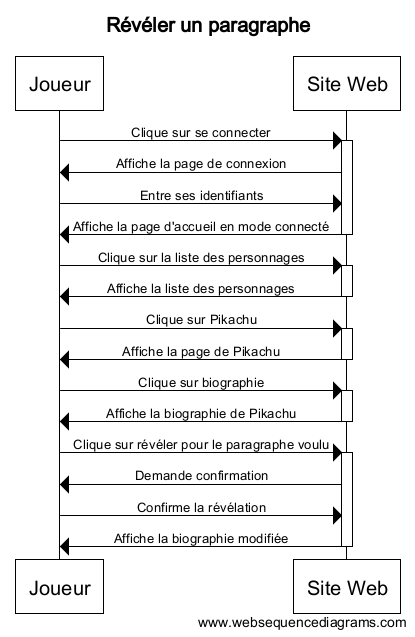
\includegraphics[scale=0.5]{sequence/RevelerParagAnalyse.png}
      \item Un joueur peut créer un personnage 
      \begin{enumerate}
        \item  Le joueur doit alors indiquer : nom, date de naissance, profession ainsi qu'une biographie initiale
        \item Le joueur peut soumettre le personnage ainsi créé à un meneur de jeu
        \item Le meneur de jeu peut accepter le personnage, il peut lire la biographie (y compris les parties secrètes).
      \end{enumerate}
      \item Le meneur de jeu, ou un joueur, peut ajouter des épisodes à la biographie d'un de ses personnages 
      \begin{enumerate}
        \item Il en spécifie la date
        \item Il peut spécifier une aventure à laquelle est rattaché cet épisode. 
        \item  Il peut sauvegarder l'épisode en cours de rédaction.
        \item Il peut reprendre l'édition.
        \item Il peut supprimer l'épisode en cours d'édition
        \item Il peut le valider
        \item Une fois validé par le joueur et le meneur de jeu l'épisode devient définitif : il ne peut plus être modifier.
      \end{enumerate}
      \textit{De ce fait il est impossible de valider un épisode si le personnage n'a pas de meneur de jeu associé.}
      \begin{center}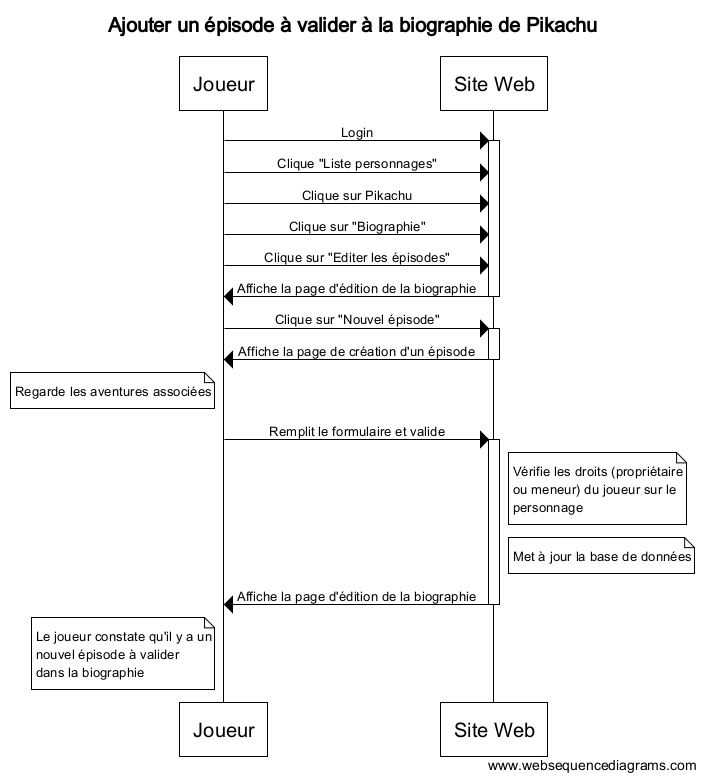
\includegraphics[scale=0.5]{sequence/AjouterEpisodeBiographie.png} \end{center}
    \item Un joueur peut proposer d'organiser une partie
    \begin{enumerate}
        \item  Il indique alors : titre, univers dans lequel se déroule la partie, situation initiale date et lieu
        \item La proposition est alors visible par tous.
        \item Le meneur de jeu peut ajouter ou enlever des personnages, ceux-ci doivent être du même univers que la partie et il doit être le meneur de jeu des personnages
        \item La proposition peut être supprimée
    \end{enumerate}
    \item Le meneur de jeu peut saisir un résumé des événements et indiquer la fin de la partie
    \begin{enumerate}
        \item Les éléments relatifs à la partie ne sont dés lors plus modifiables.
        \item La partie devient une aventure pouvant apparaitre dans la biographie des personnages.
    \end{enumerate}
    \item Un joueur peut céder son personnage
    \begin{enumerate}
        \item Il indique le joueur bénéficiaire
    \end{enumerate}
    \item Un joueur peut changer le meneur de jeu d'un de ses personnages
    \begin{enumerate}
        \item Le nouveau meneur de jeu doit accepter.
        \item Ce transfert ne peut avoir lieu que si le personnage n'est pas impliqué dans une partie en cours.
    \end{enumerate}
    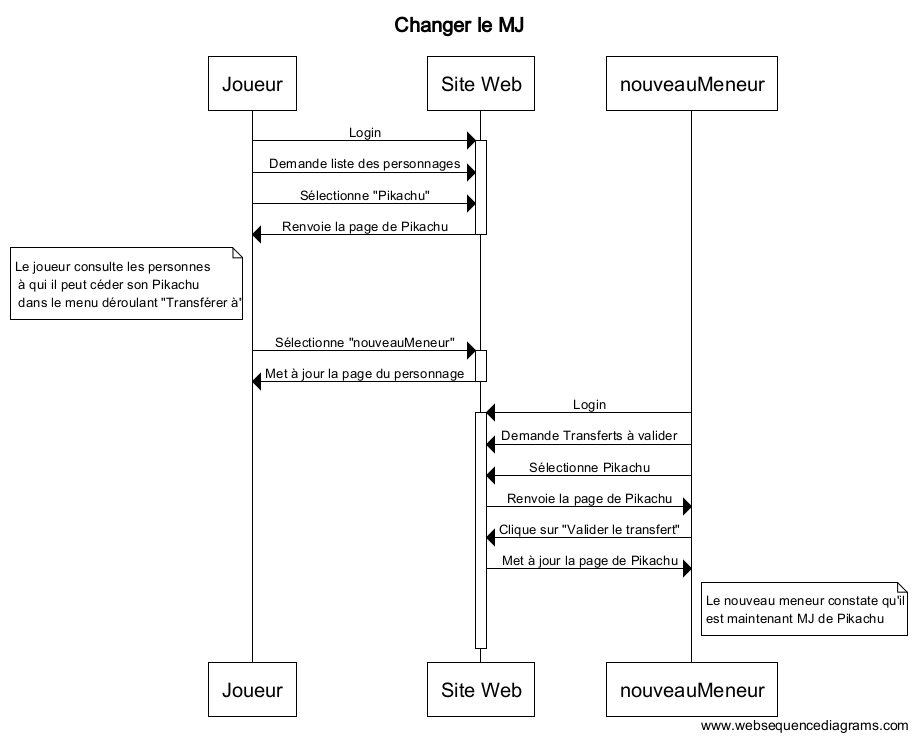
\includegraphics[scale=0.5]{sequence/ChangerleMJ.png}
    \end{enumerate}

\subsubsection{Diagramme des cas d'utilisation}

\begin{center}
    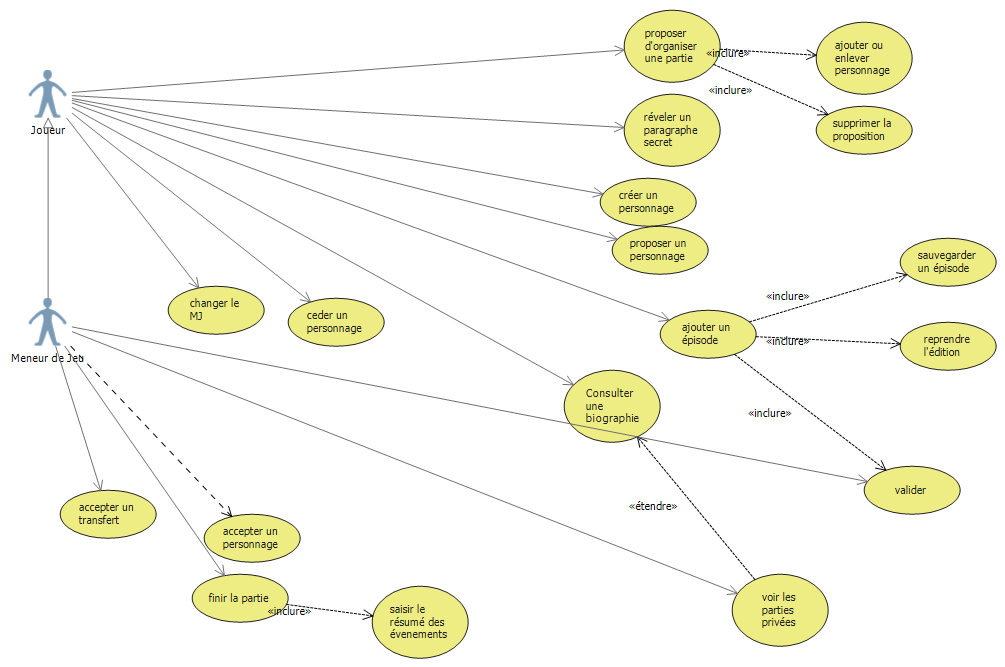
\includegraphics[scale=0.7,angle=90]{analyse/usecases}
\end{center}

\subsection{Diagramme de classes d'analyse}
Le sujet fournit une description des différents "objets" de l'application : partie, aventure, personnage, univers, biographie, épisode, paragraphe ... 
Voici le diagramme de classe d'analyse que nous en avons tiré.\\
\textit{Nous avons considéré qu'une partie était simplement une aventure en cours (nous aurions pu faire de l'héritage mais l'avantage semblait mince par rapport aux inconvénients de la conversion d'une partie en aventure ). \\
    De même nous n'avons pas distingués les classes joueur et meneur de jeu : un joueur est meneur de jeu s'il est engagé dans les relations qui caractérisent un meneur de jeu (parties menés, personnages dont il est le meneur ...) Cela se justifie par le caractère dynamique de ce  statut : un joueur peut facilement devenir meneur de jeu ou arrêter de l'être, être un meneur de jeu semblait donc être plutôt une propriété dynamique des joueurs. }
\begin{center}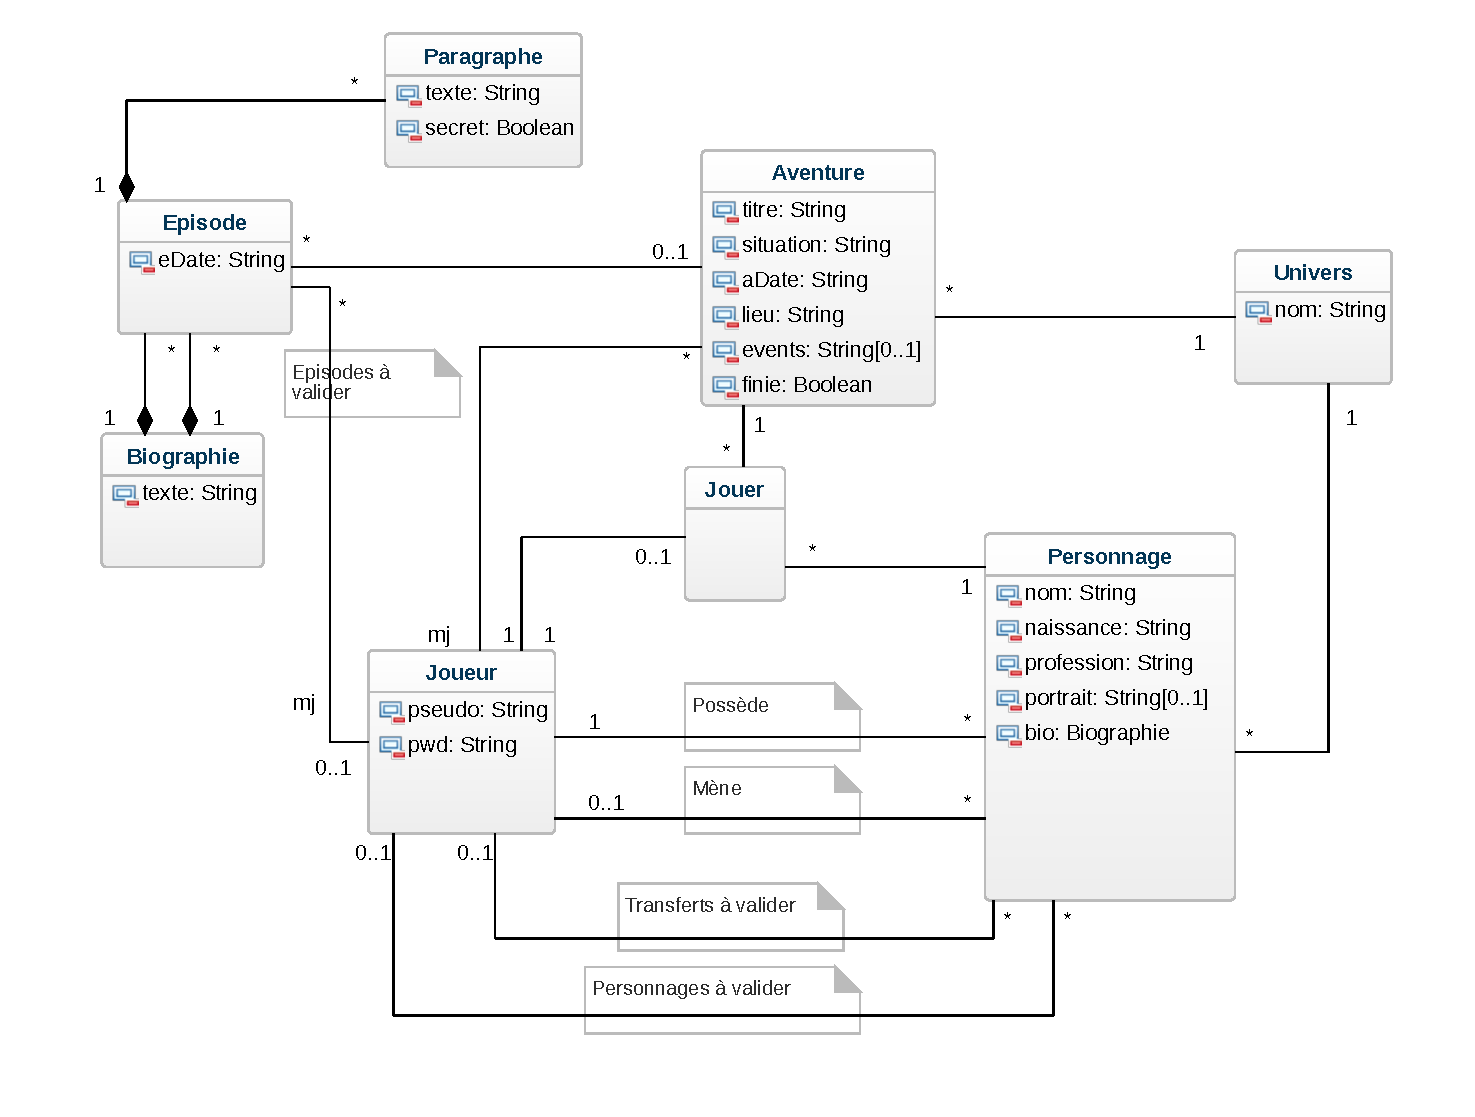
\includegraphics[scale=0.7]{analyse/classes.pdf} \end{center}







% (b) Document de conception :
% — L’architecture générale modèle-vue-contrôleur est imposée, mais indiquez comment vous la
% mettez en œuvre : quels sont les contrôleurs et les vues, comment tout s’articule-t-il.
% — Conception détaillée : diagramme de classes logicielles, diagrammes de séquence, diagrammes
% d’états-transitions si cela est pertinent. Ces diagrammes doivent être cohérents entre eux et
% avec l’implémentation. Il est inutile de fournir des diagrammes illisibles ou qui n’apportent
% aucune information ; il peut être en revanche utile d’ajouter un minimum de texte explicatif
% le cas échéant.

\section {Conception}



\section {Détails techniques}

L'application est normalement protégée contre tout type de faille XSS (via JSTL) et également des attaques par injection SQL.

De plus la vérification des droits d'accès pour chaque type d'action a bien été implémentée, ainsi que la gestion des différentes erreurs dont le message reste intégré au design de l'application.


\section {Manuel d'utilisation}



% (d) Bilan sur les outils de modélisation utilisés, en particulier les problèmes rencontrés, ainsi que
% les solutions trouvées. Il vous est demandé dans cette partie de bien préciser les logiciels, en particulier les modeleurs UML que vous avez utilisés.

\section {Bilan}





\end{document}


